\documentclass[a5paper,12pt]{article}
\usepackage[utf8]{inputenc}
\usepackage[T1]{fontenc}
\usepackage{graphicx}
\usepackage{geometry}
\usepackage{multicol}

% Page setup for A5 booklet printing
\geometry{a5paper, margin=1.2cm}
\setlength{\parskip}{0.5em}
\setlength{\parindent}{0pt}
\setlength{\columnsep}{1em}

\begin{document}

% Title Page
\begin{titlepage}
\centering
\vspace*{1cm}
{\LARGE\bfseries Asseily Carols}\\[1cm]
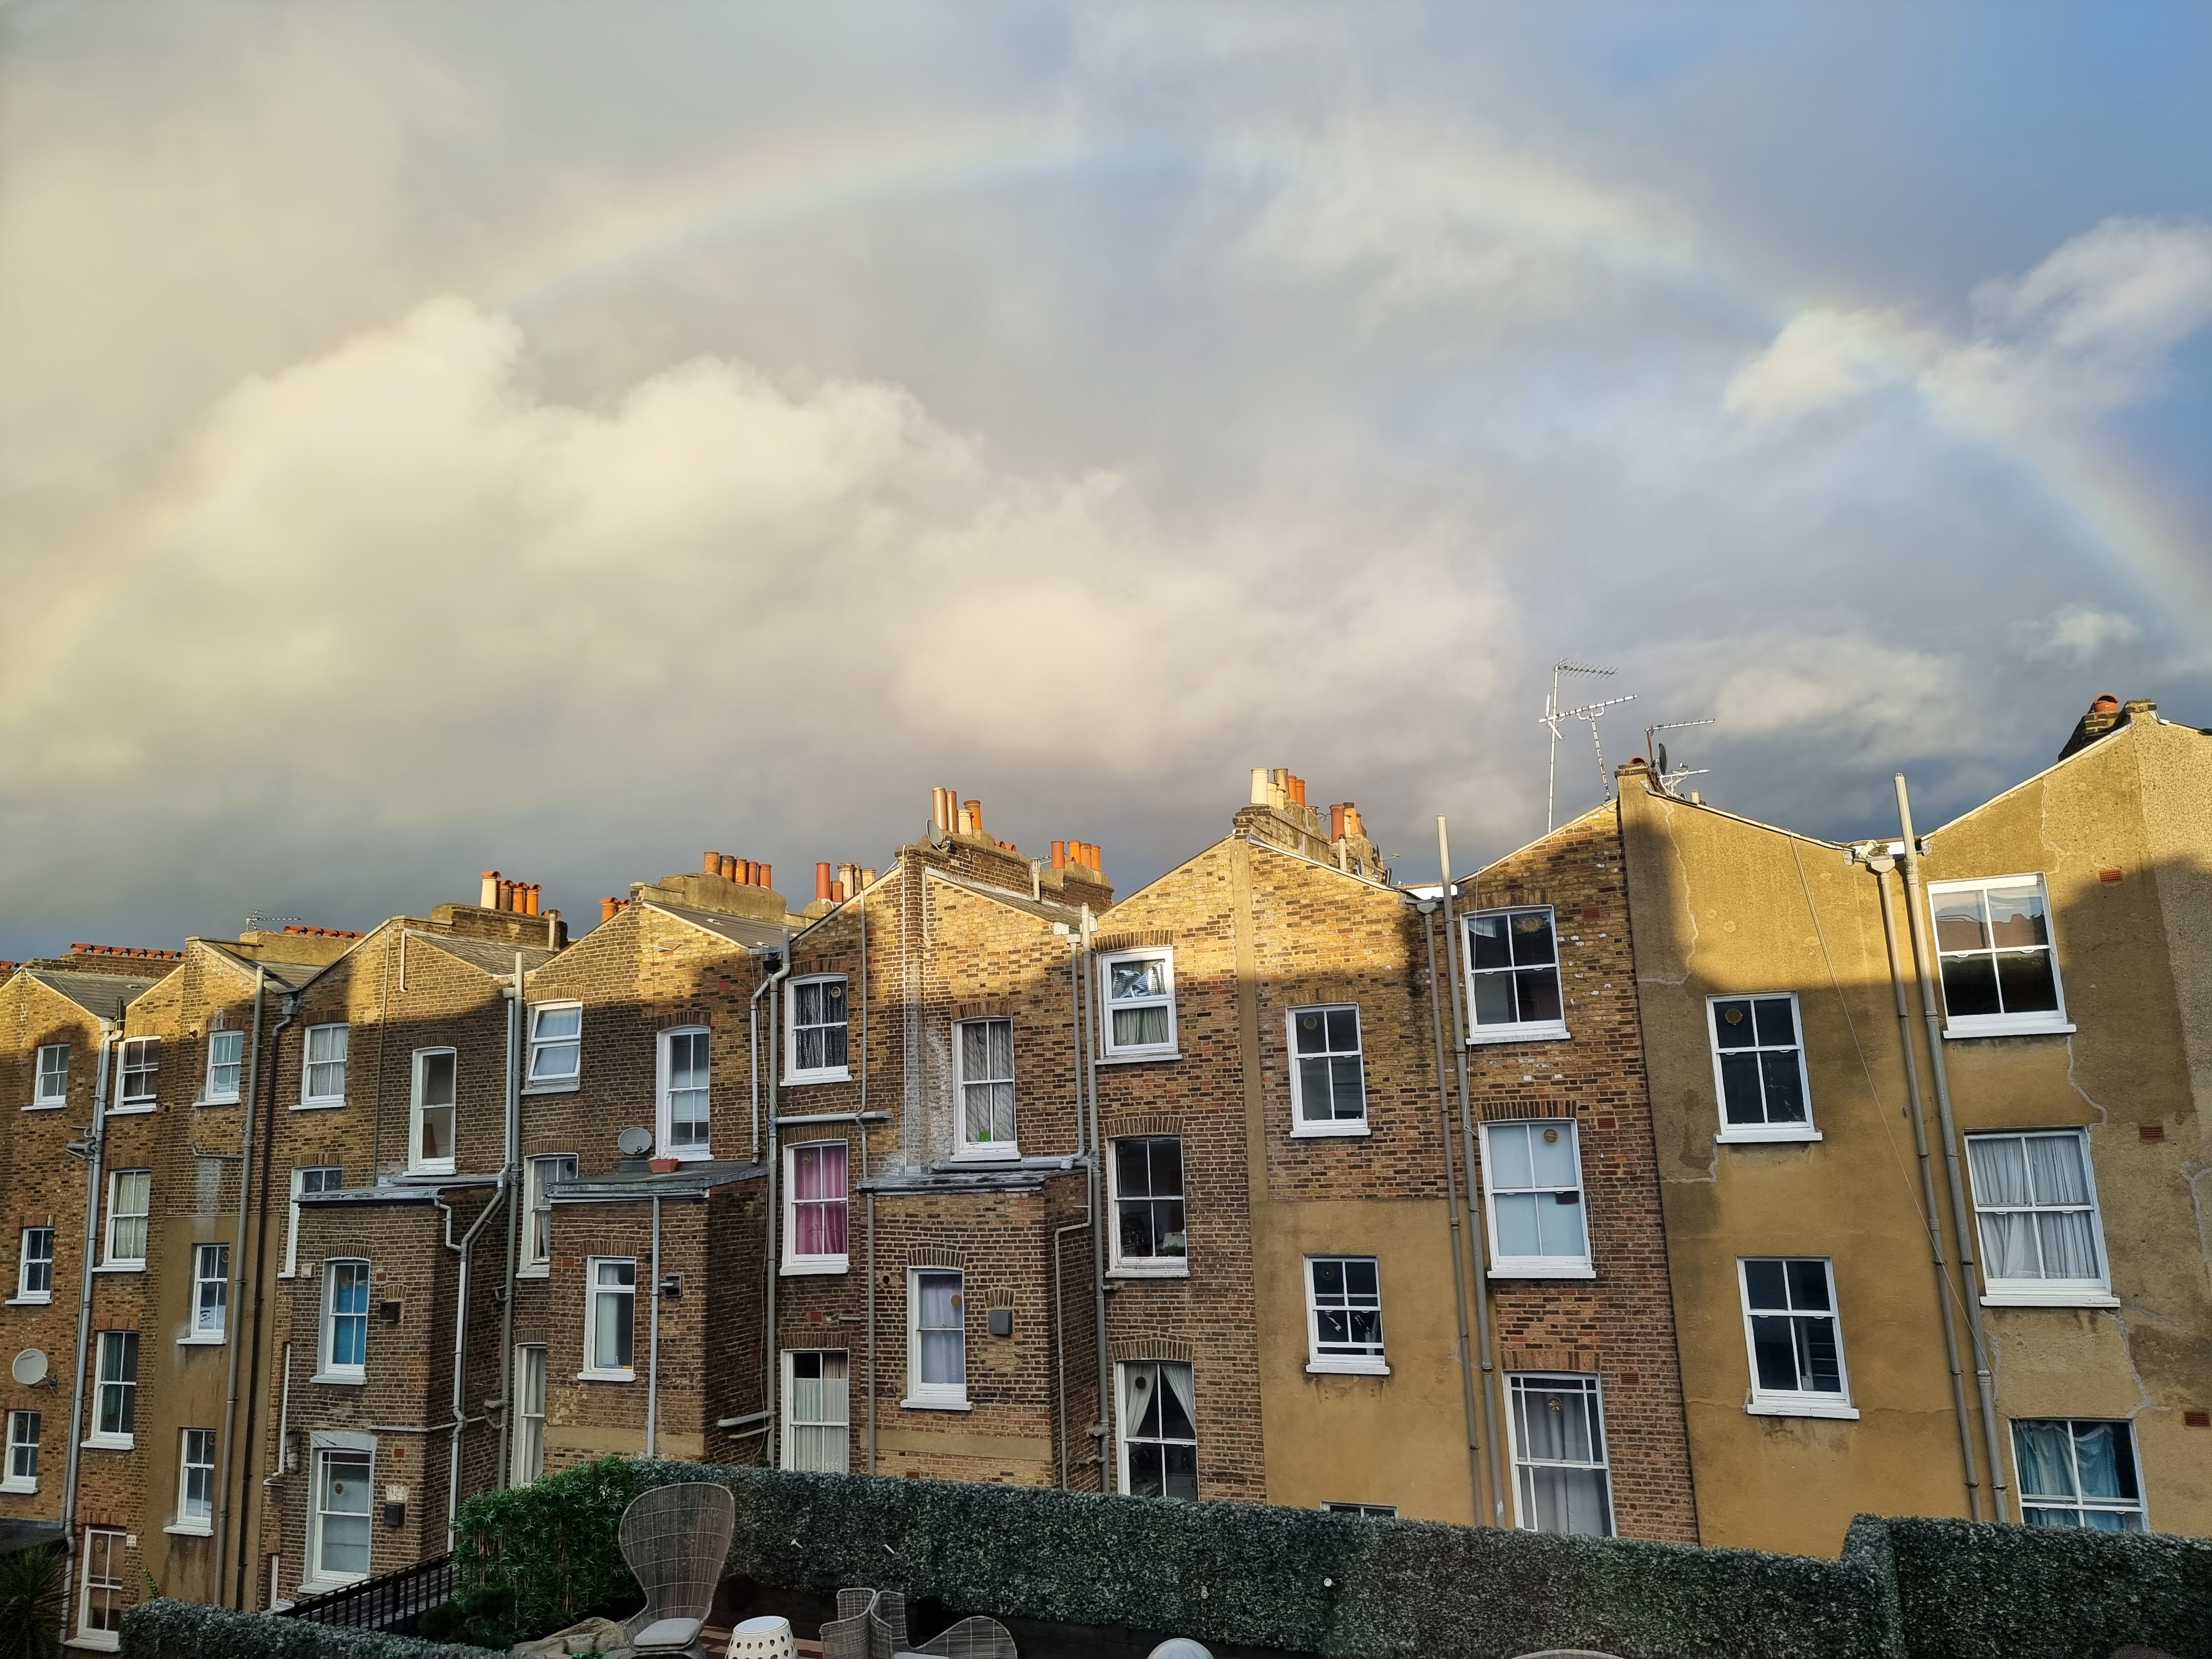
\includegraphics[width=0.9\textwidth]{20211212.jpg}\\[1cm]
\vfill
\end{titlepage}

\begin{center}{\Large\bfseries Silent Night}\end{center}
\vspace{0.3em}
\textbf{1.} Silent night! Holy night!\\
All is calm, all is bright.\\
Round yon Virgin Mother and Child\\
Holy Infant so tender and mild,\\
Sleep in heavenly peace,\\
Sleep in heavenly peace.

\textbf{2.} Silent night! Holy night!\\
Shepherds quake at the sight\\
Glories stream from heaven afar\\
Heavenly hosts sing Alleluia!\\
Christ the saviour is born,\\
Christ the saviour is born.

\textbf{3.} Silent night! Holy night!\\
Son of God, love's pure light\\
Radiant beams from thy holy face\\
With the dawn of redeeming grace,\\
Jesus, Lord, at thy birth!\\
Jesus, Lord, at thy birth!

\newpage

\begin{center}{\Large\bfseries While Shepherds Watched}\end{center}
\vspace{0.3em}
\textbf{1.} While shepherds watched their flocks by night,\\
All seated on the ground,\\
The angel of the Lord came down,\\
And glory shone around.

\textbf{2.} 'Fear not,' said he for mighty dread\\
Had siezed their troubled mind;\\
'Glad tidings of great joy I bring\\
To you and all mankind.

\textbf{3.} 'To you, in David's town, this day\\
Is born of David's line\\
A Saviour, who is Christ the Lord;\\
And this shall be the sign:

\begin{multicols}{2}
\small
\textbf{4.} 'The heavenly Babe you there shall find\\
To human view displayed,\\
All meanly wrapped in swathing bands,\\
And in a manger laid.'

\textbf{5.} Thus spake the seraph; and forthwith\\
Appeared a shining throng\\
Of angels, praising God, who thus\\
Addressed their joyful song:

\textbf{6.} 'All glory be to God on high,\\
And to the earth be peace;\\
Good will henceforth from heaven to men\\
Begin, and never cease!'

\end{multicols}
\newpage

\begin{center}{\Large\bfseries In the Bleak Mid-Winter}\end{center}
\vspace{0.3em}
\textbf{1.} In the bleak midwinter\\
Frosty wind made moan,\\
Earth stood hard as Iron,\\
Water like a stone;\\
Snow had fallen, snow on snow,\\
Snow on snow,\\
In the bleak midwinter\\
Long ago.

\textbf{2.} Our God, Heav'n cannot hold Him\\
Nor earth sustain;\\
Heav'n and earth shall flee a way\\
When He comes to reign;\\
In the bleak midwin ter\\
A stable place-sufficed\\
The Lord God Almighty\\
Jesus Christ.

\textbf{3.} E nough for Him, whom cheru bim\\
Worship night and day,\\
A breast -ful of milk And\\
a mangerful of hay;\\
Enough for Him, whom an -gels\\
Fall down-before,\\
The ox and ass and camel\\
Which adore.

\begin{multicols}{2}
\small
\textbf{4.} Angels and archangels\\
May have gathered there,\\
Cherubim and sera-phim\\
Thronged . the air;\\
But on -ly His Mo -ther\\
In her maiden bliss\\
Worshipped the Beloved\\
With a kiss.

\textbf{5.} What can I give Him,\\
Poor as I am?\\
If I were a shepherd\\
I would bring a lamb,\\
If I were a Wise Man\\
I-would do-my part,\\
Yet what I can I give Him,\\
Give my heart.

\end{multicols}
\newpage

\begin{center}{\Large\bfseries Away In A Manger}\end{center}
\vspace{0.3em}
\textbf{1.} Away in a manger, no crib for a bed,\\
The little Lord Jesus laid down His sweet head,\\
The stars in the bright sky looked down where He lay,\\
The little Lord Jesus asleep on the hay.

\textbf{2.} The cattle are lowing, the Baby awakes,\\
But little Lord Jesus no crying He makes;\\
I love Thee, Lord Jesus; look down from the sky,\\
And stay by my bedside till morning is nigh.

\textbf{3.} Be near me, Lord Jesus, I ask Thee to stay\\
Close by me forever, and love me I pray.\\
Bless all the dear children in Thy tender care,\\
And fit us for heaven, to live with Thee there.

\newpage

\begin{center}{\Large\bfseries Good King Wenceslas}\end{center}
\vspace{0.3em}
\textbf{1.} Good King Wenceslass looked out\\
On the feast of Stephen,\\
When the snow lay round about,\\
Deep and crisp and even;\\
Brightly shone the moon that night,\\
Though the frost was cruel;\\
When a poor man came in sight\\
Gath'ring winter fuel.

\textbf{2.} ''Hither, page, and stand by me,\\
If thou know'st it, telling,\\
Yonder peasant, who is he;\\
Where and what his dwelling?''\\
''Sire, he lives a good league hence,\\
Underneath the mountain,\\
Right against the forest fence,\\
By Saint Agnes' fountain.

\textbf{3.} ''Bring me flesh and bring me wine;\\
Bring me pine logs hither.\\
Thou and I will see him dine,\\
When we bear them thither.''\\
Page and monarch, forth they went;\\
Forth they went together\\
Through the rude wind's wild lament\\
And the bitter weather.

\begin{multicols}{2}
\small
\textbf{4.} ''Sire, the night is darker now,\\
And the wind blows stronger;\\
Fails my heart, I know not how;\\
I can go no longer.''\\
''Mark my footsteps, good my page,\\
Tread thou in them boldly;\\
Thou shalt find the winter's rage\\
Freeze thy blood less coldly.''

\textbf{5.} In his master's steps he trod,\\
Where the snow lay dinted;\\
Heat was in the very sod\\
Which the saint had printed.\\
Therefore, Christian men, be sure,\\
Wealth or rank possessing,\\
Ye who now will bless the poor,\\
Shall yourselves find blessing.

\end{multicols}
\newpage

\begin{center}{\Large\bfseries Once In Royal David's City}\end{center}
\vspace{0.3em}
\textbf{1.} Once in royal David's city\\
Stood a lowly cattle shed,\\
Where a mother laid her baby\\
In a manger for His bed:\\
Mary was that mother mild\\
Jesus Christ her little Child.

\textbf{2.} He came down to earth from heaven\\
Who is God and Lord of all,\\
And His shelter was a stable\\
And his cradle was a stall;\\
With the poor, and mean, and low-ly\\
Lived on earth our Saviour holy.

\textbf{3.} And, through all His wondrous childhood\\
He would honour and obey,\\
Love, and watch the lowly maiden\\
In whose gentle arms He lay:\\
Christian children all must be\\
Mild, Obedient, good as He.

\begin{multicols}{2}
\small
\textbf{4.} For He is our childhood's pattern,\\
Day by day like us He grew;\\
He was little, weak, and helpless,\\
Tears and smiles like us He knew;\\
And He feeleth for our sad-ness,\\
And He shareth in our glad-ness

\textbf{5.} And our eyes at last shall see Him,\\
Through His own redeeming love,\\
For that Child so dear and gentle\\
Is our Lord in heaven above;\\
And He leads His children on\\
To the place where He is gone.

\textbf{6.} Not in that poor lowly stable,\\
With the oxen standing by,\\
We shall see Him; but in heaven,\\
Set at God's right hand on high;\\
When like stars His children crowned\\
All in white shall wait around.

\end{multicols}
\newpage

\begin{center}{\Large\bfseries O Little Town of Bethlehem}\end{center}
\vspace{0.3em}
\textbf{1.} O little town of Bethlehem\\
How still we see thee lie;\\
Above thy deep and dreamless sleep\\
The silent stars go by:\\
Yet in thy dark streets shineth\\
The everlasting Light;\\
The hopes and fears of all the years\\
Are met in thee tonight.

\textbf{2.} For Christ is born of Ma ry;\\
And gathered all above,\\
While mortals sleep, the angels keep\\
Their watch of wondering love.\\
O morning stars, together\\
Proclaim the holy birth,\\
An praises sing to God the King,\\
And peace to men on earth!

\textbf{3.} How silently, how si-lently\\
The wondrous gift is giv'n!\\
So God imparts to human hearts\\
The blessings of His heaven:\\
No ear may hear His coming;\\
But in this world of sin,\\
Where meek souls will receive Him, still\\
The dear Christ enters in.

\begin{multicols}{2}
\small
\textbf{4.} O Holy Child of Beth-lehem,\\
Descend to us we pray;\\
Cast out our sin, and enter in;\\
Be born in us today.\\
We hear the heavenly angels\\
The great glad tidings tell:\\
O come to us, abide with us,\\
Our Lord Emmanuel.

\end{multicols}
\newpage

\begin{center}{\Large\bfseries Hark the Herald Angels Sing}\end{center}
\vspace{0.3em}
\textbf{1.} Hark! the herald angels sing,\\
Glory to the new born King,\\
Peace on earth, and mercy mild,\\
God and sinners reconciled.\\
Joyful all ye nations, rise,\\
Join the triumph of the skies;\\
With the-angelic host proclaim\\
'Christ is born in Bethlehem.'\\
Hark! the herald angels sing,\\
Glory to the new born King,

\textbf{2.} Christ, by highest heaven adored,\\
Christ, the everlasting Lord\\
Late in time behold Him come,\\
Offspring of a Virgin's womb.\\
Veiled in flesh the Godhead see!\\
Hail, the-Incarnate Deity!\\
Pleased as Man with man to dwell,\\
Jesus, our Emmanuel.

\textbf{3.} Hail the heaven born Prince of peace!\\
Hail, the Sun of righteousness!\\
Light and life to all He brings,\\
Ris'n with healing in His wings.\\
Mild He lays His glory by,\\
Born that man no more may die,\\
Born to raise the sons of earth,\\
Born to give them second birth.

\newpage

\begin{center}{\Large\bfseries O Come All Ye Faithful}\end{center}
\vspace{0.3em}
\textbf{1.} O come, all ye faithful, Joyful and triumphant,\\
O come ye, O come ye to Bethlehem;\\
Come and behold Him Born the King of Angels:\\
O come, let us adore Him,\\
O come, let us adore Him,\\
O come, let us adore Him, Christ the Lord!

\textbf{2.} God of God, Light of Light,\\
Lo, He abhors not the Virgin's womb;\\
Very God, Begotten, not created;

\textbf{3.} Sing, choirs of angels, Sing in exultation,\\
Sing, all ye ci-tizens of heav'n above,\\
Glory to God In the highest;

\begin{multicols}{2}
\small
\textbf{4.} See how the Shepherds, summoned to His cradle,\\
Leaving their flocks-draw nigh with lowly fear;\\
We too will thither Bend our joyful footsteps;

\textbf{5.} Yea, Lord, we greet Thee, Born this happy morning,\\
Jesu, to Thee be glory given;\\
Word of the Father, Now in flesh appearing;

\textbf{6.} Lo! starled chieftains, Maji, Christ adoring\\
Offer Him frank-incense and gold and myrrh;\\
We to the Christ Child Bring our hearts' oblations:

\end{multicols}
\newpage

\begin{center}{\Large\bfseries The Twelve Days of Christmas}\end{center}
\vspace{0.3em}
\textbf{1.} On the first day of Christmas my true love gave to me\\
A partridge in a pear tree.

\textbf{2.} On the second day of Christmas my true love gave to me\\
Two turtle doves,\\
And a partridge in a pear tree.

\textbf{3.} On the third day of Christmas my true love gave to me\\
Three French hens,\\
Two turtle doves,\\
And a partridge in a pear tree.

\begin{multicols}{2}
\small
\textbf{4.} On the fourth day of Christmas my true love gave to me\\
Four calling birds,\\
Three French hens,\\
Two turtle doves,\\
And a partridge in a pear tree.

\textbf{5.} On the fifth day of Christmas my true love gave to me\\
Five golden rings,\\
Four calling birds,\\
Three French hens,\\
Two turtle doves,\\
And a partridge in a pear tree.

\textbf{6.} On the sixth day of Christmas my true love gave to me\\
Six geese a-laying,\\
Five golden rings,\\
Four calling birds,\\
Three French hens,\\
Two turtle doves,\\
And a partridge in a pear tree.

\textbf{7.} On the seventh day of Christmas my true love gave to me\\
Seven swans a-swimming,\\
Six geese a-laying,\\
Five golden rings,\\
Four calling birds,\\
Three French hens,\\
Two turtle doves,\\
And a partridge in a pear tree.

\textbf{8.} On the eighth day of Christmas my true love gave to me\\
Eight maids a-milking,\\
Seven swans a-swimming,\\
Six geese a-laying,\\
Five golden rings,\\
Four calling birds,\\
Three French hens,\\
Two turtle doves,\\
And a partridge in a pear tree.

\textbf{9.} On the ninth day of Christmas my true love gave to me\\
Nine ladies dancing,\\
Eight maids a-milking,\\
Seven swans a-swimming,\\
Six geese a-laying,\\
Five golden rings,\\
Four calling birds,\\
Three French hens,\\
Two turtle doves,\\
And a partridge in a pear tree.

\textbf{10.} On the tenth day of Christmas my true love gave to me\\
Ten lords a-leaping,\\
Nine ladies dancing,\\
Eight maids a-milking,\\
Seven swans a-swimming,\\
Six geese a-laying,\\
Five golden rings,\\
Four calling birds,\\
Three French hens,\\
Two turtle doves,\\
And a partridge in a pear tree.

\textbf{11.} On the eleventh day of Christmas my true love gave to me\\
Eleven pipers piping,\\
Ten lords a-leaping,\\
Nine ladies dancing,\\
Eight maids a-milking,\\
Seven swans a-swimming,\\
Six geese a-laying,\\
Five golden rings,\\
Four calling birds,\\
Three French hens,\\
Two turtle doves,\\
And a partridge in a pear tree.

\textbf{12.} On the twelfth day of Christmas my true love gave to me\\
Twelve drummers drumming,\\
Eleven pipers piping,\\
Ten lords a-leaping,\\
Nine ladies dancing,\\
Eight maids a-milking,\\
Seven swans a-swimming,\\
Six geese a-laying,\\
Five golden rings,\\
Four calling birds,\\
Three French hens,\\
Two turtle doves,\\
And a partridge in a pear tree!

\end{multicols}

\end{document}
